\section{Sequences}
In this sections the important processes of the system are shown exemplarily. This includes a request 
from the web page which is handled in the web server tier, any call on the facade of the application tier,
a parsing process and a chart request.

\subsection{HTTP request}
A HTTP request is triggered by the user on the web page.

BILD vll genaues beispiel und dan methodenname noch in beschreibung

\subsection{Facade call}
In the following sequence diagram a call on the application tier facade is shown 
on the example of a chart request with \texttt{computeChart(..)}.



\subsection{Chart request}
Sequence diagram of a \texttt{computeChart(..)} call, a chart request, on the ChartMediator.

BILD


\subsection{Parsing}
This activity diagram shows the generell work flow of a parsing process of a log file. 
The sequence diagram underneath describes this proess with the point of view on the 
interaction of the classes.

AKTIVITY-PIC

\begin{center}
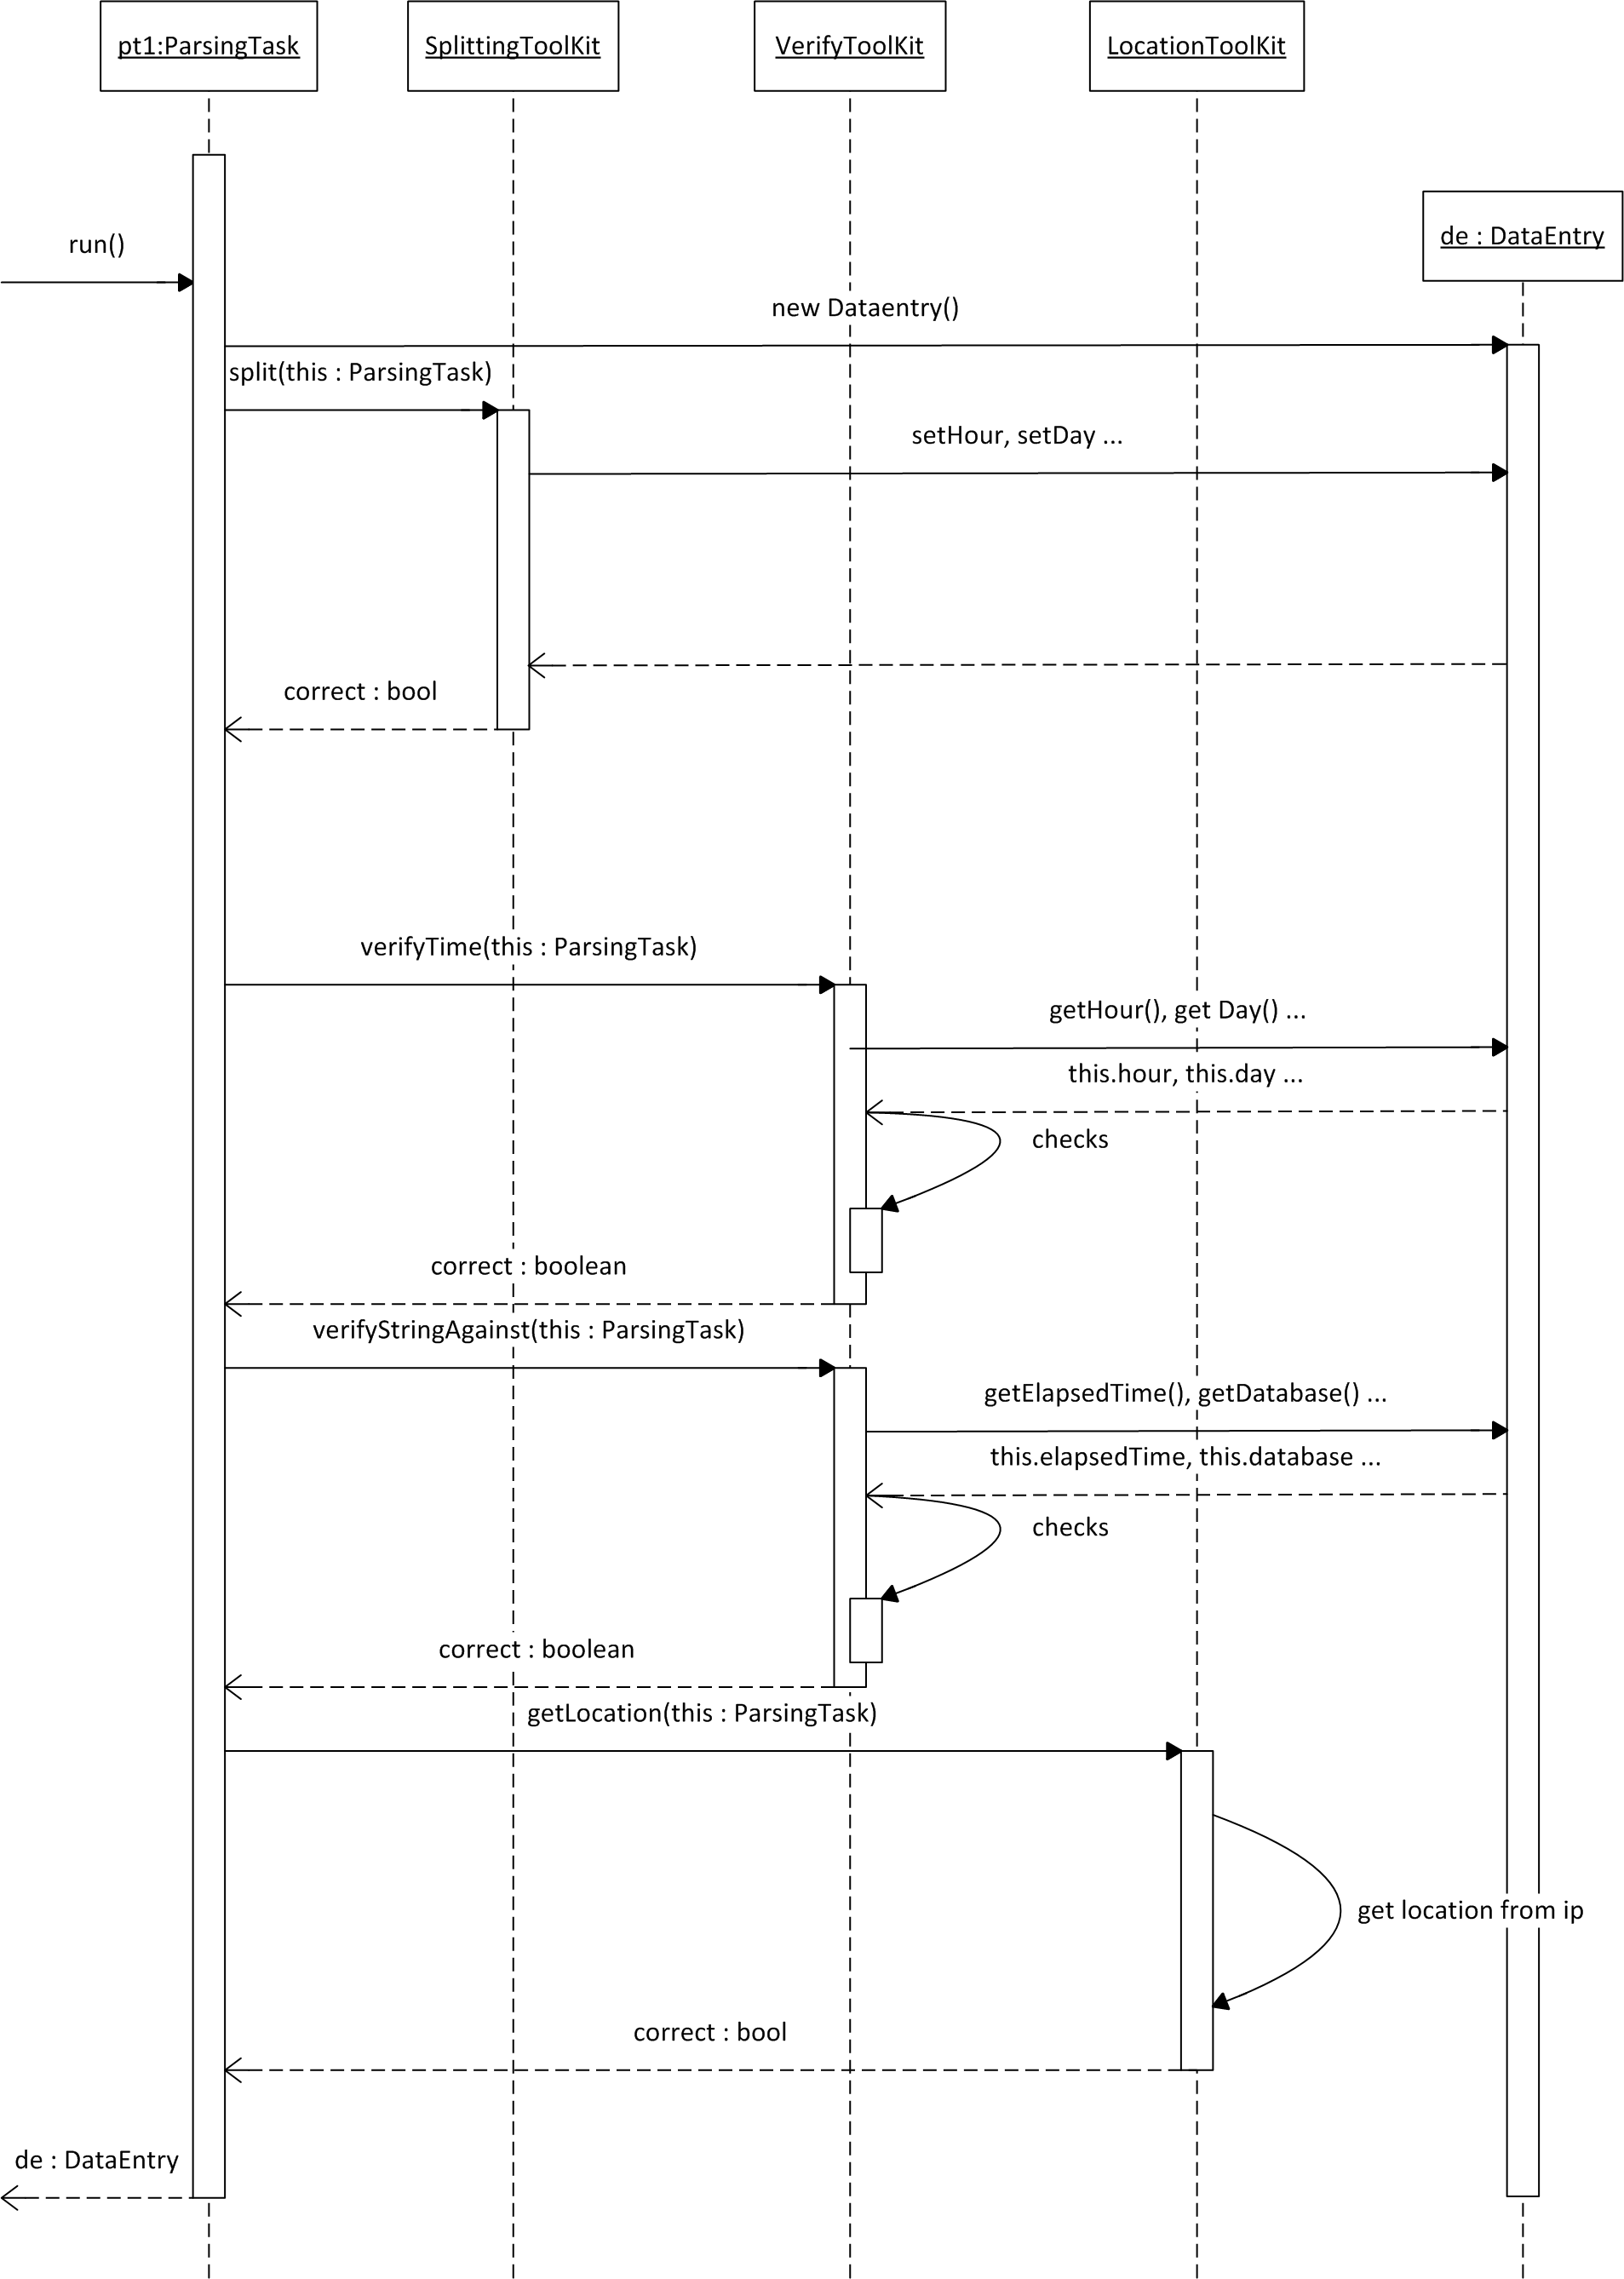
\includegraphics[width=0.7\linewidth]{Pictures/Seq/SeqParser.png}
\end{center}



   
